%% LyX 1.6.5 created this file.  For more info, see http://www.lyx.org/.
%% Do not edit unless you really know what you are doing.
\documentclass[11pt,ngerman,pointlessnumbers,DIV10,BCOR10mm,tocleft,utf8]{scrreprt}
\usepackage[T1]{fontenc}
\setcounter{secnumdepth}{3}
\setcounter{tocdepth}{3}
\usepackage{float}
\usepackage{graphicx}

\makeatletter
%%%%%%%%%%%%%%%%%%%%%%%%%%%%%% User specified LaTeX commands.
\setcounter{tocdepth}{2} 
%\typearea[5mm]{13}

% --- ALLGEMEINES; EINGABE; ZEICHEN ---
%\usepackage[T1]{fontenc}
\usepackage[utf8]{inputenc}
\usepackage[ngerman]{babel}
\usepackage{amssymb,amsmath,amsfonts,stmaryrd}
\usepackage{wasysym,relsize}

% --- INDEX ---
\usepackage{makeidx}
\makeindex

% --- DIVERSES ---
\usepackage{graphicx}
\usepackage{enumerate}


% --- FARBEN UND PSTRICKS ---
\usepackage{color,pstricks}
\newgray{gray}{0.25}
\newgray{komagray}{0.4}
\newgray{lightgray}{0.45}
\newgray{verylightgray}{0.65}
\newgray{verydarkgray}{0.15}
\newrgbcolor{green}{0 0.75 0}

% --- TITELFARBEN ---
\newrgbcolor{screenblue} {0.588 0.667 0.745}
\newrgbcolor{Screenblue} {0.275 0.431 0.667}
\newrgbcolor{dekoblue}   {0.392 0.588 0.863}
\newrgbcolor{screenbrown}{0.851 0.851 0.816}
\newrgbcolor{Screenbrown}{0.824 0.824 0.784}
\newrgbcolor{SCREENBROWN}{0.745 0.745 0.725}
\newrgbcolor{dekobrown}  {0.686 0.686 0.667}
\newrgbcolor{Dekobrown}  {0.667 0.667 0.647}
\newrgbcolor{printcolor} {0.195 0.195 0.195}

% --- KOMA-ANPASSUNGEN ---
\newgray{komagray}{0.4}
\addtokomafont{sectioning}{\komagray}
\setkomafont{pagehead}{\normalfont\komagray\large\sffamily}
\addtokomafont{pagenumber}{\usekomafont{pagehead}}
\addtokomafont{footnote}{\komagray}

% --- ANPASSUNGEN ---
\renewcommand{\labelitemi}{$\circ$}
\renewcommand{\labelenumi}{(\arabic{enumi})}
\renewcommand{\labelenumii}{(\roman{enumii})}
\renewcommand{\labelenumiii}{(\alph{enumiii})}
% --- LAENGEN-ANPASSUNGEN ---
\setlength{\parindent}{0pt}
\setlength{\parskip}{1.6ex plus 0.2ex minus 0.2ex}
\psset{unit=1cm}
% pakete laden, werte einstellen
%inhaltszähler
\newcounter{content}[chapter]
\newcounter{subcontent}[content]

%inhaltstyp
\newcommand{\contenttype}[2]{%
\stepcounter{content}%
\subsection*{#2 \thechapter.\thecontent: #1}%
\addcontentsline{toc}{subsection}{\numberline{}#2 \thechapter.\thecontent: #1}}

% inhalte
\newcommand{\definition}[1]{\contenttype{#1}{Definition}}
\newcommand{\proposition}[1]{\contenttype{#1}{Proposition}}
\newcommand{\lemma}[1]{\contenttype{#1}{Lemma}}
\newcommand{\korollar}[1]{\contenttype{#1}{Korollar}}
\newcommand{\satz}[1]{\contenttype{#1}{Satz}}
\newcommand{\folgerung}[1]{\contenttype{#1}{Folgerung}}
\newcommand{\beispiel}[1]{\contenttype{#1}{Beispiel}}


%unterinhaltstyp
\newcommand{\subcontenttype}[2]{%
\stepcounter{subcontent}%
\subsection*{#2 \thechapter.\thecontent.\alph{subcontent}: #1}%
\addcontentsline{toc}{subsection}{\numberline{}#2 \thechapter.\thecontent.\alph{subcontent}: #1}}

%subinhalte
\newcommand{\subdefinition}[1]{\subcontenttype{#1}{Definition}}
\newcommand{\subproposition}[1]{\subcontenttype{#1}{Proposition}}
\newcommand{\sublemma}[1]{\subcontenttype{#1}{Lemma}}
\newcommand{\subkorollar}[1]{\subcontenttype{#1}{Korollar}}
\newcommand{\subsatz}[1]{\subcontenttype{#1}{Satz}}
\newcommand{\subfolgerung}[1]{\subcontenttype{#1}{Folgerung}}
\newcommand{\subbeispiel}[1]{\subcontenttype{#1}{Beispiel}}


%weitere strukturen
\newcommand{\bsp}[1]{\subsubsection*{Beispiel: #1}}
\newcommand{\bsps}[1]{\subsubsection*{Beispiele: #1}}
\newcommand{\beweis}{\subsubsection*{Beweis:}}
\newcommand{\bemerkung}{\subsubsection*{Bemerkung:}}


%für aufgabenzettel und lösungen
\newcounter{series}
\newcounter{task}[series]

\newcommand{\series}{
\stepcounter{series}%
\section*{Serie \theseries}%
\addcontentsline{toc}{section}{\numberline{}{Serie \theseries}}}

\newcommand{\task}{\stepcounter{task}\subsection*{Aufgabe \thetask}\vspace{-2ex}\markright{Aufgabe \thetask}}
\newcommand{\solution}{\subsubsection*{Beweis:}}

% eigene befehle
%mengen u.s.w
\newcommand{\pmenge}{\mathcal{P}}
\newcommand{\setN}{\mathbb{N}}
\newcommand{\setR}{\mathbb{R}}
\newcommand{\setQ}{\mathbb{Q}}
\newcommand{\setE}{\mathbb{E}}

% abkuerzuungen
\newcommand{\w}{\omega}

\newcommand{\wkeit}{\ensuremath{\,\mathbb{P}}}
\newcommand{\Wkeit}{Wahrscheinlichkeit{ }}

\newcommand{\wmas}{\ensuremath{\,\mathbb{P}}}
\newcommand{\Wmas}{Wahrscheinlichkeitsmaß{ }}

\newcommand{\wraum}{\ensuremath{(\varOmega, \varSigma, \mathbb{P})}{ }}
\newcommand{\Wraum}{Wahrscheinlichkeitsraum{ }}

%operatoren 
\newcommand{\var}{\mathrm{\,Var}}
\newcommand{\cov}{\mathrm{\,Cov}}
\newcommand{\vol}{\mathrm{\,Vol}}
\newcommand{\ber}{\mathrm{\,Ber}}
\newcommand{\bin}{\mathrm{\,Bin}}
\newcommand{\geom}{\mathrm{\,Geom}}
\newcommand{\poi}{\mathrm{\,Poi}}

%große operatoren mit \limits
\newcommand{\Int}{\textstyle\int\limits}
\newcommand{\Sum}{\textstyle\sum\limits}
\newcommand{\Prod}{\textstyle\prod\limits}
\renewcommand{\Cup}{\textstyle\bigcup\limits}
\renewcommand{\Cap}{\textstyle\bigcap\limits}

%deutsche anführungszzeichen
\newcommand{\gqq}[1]{\glqq{#1\grqq}}
\newcommand{\gq}[1]{\glq{#1\grq}}% eigene mathe-befehle


\renewcommand{\thesection}{\arabic{section}}\renewcommand{\thefigure}{\arabic{figure}}\newcommand{\token}[1]{\ensuremath{\text{\texttt{\,{#1}\,}}}}

\makeatother



\begin{document}

\chapter*{Software-Challenge 2011}

\vspace*{-0.9cm}
 


\section*{Spielanleitung zu ,,Sch\"{a}fchen im Trockenen{}``}

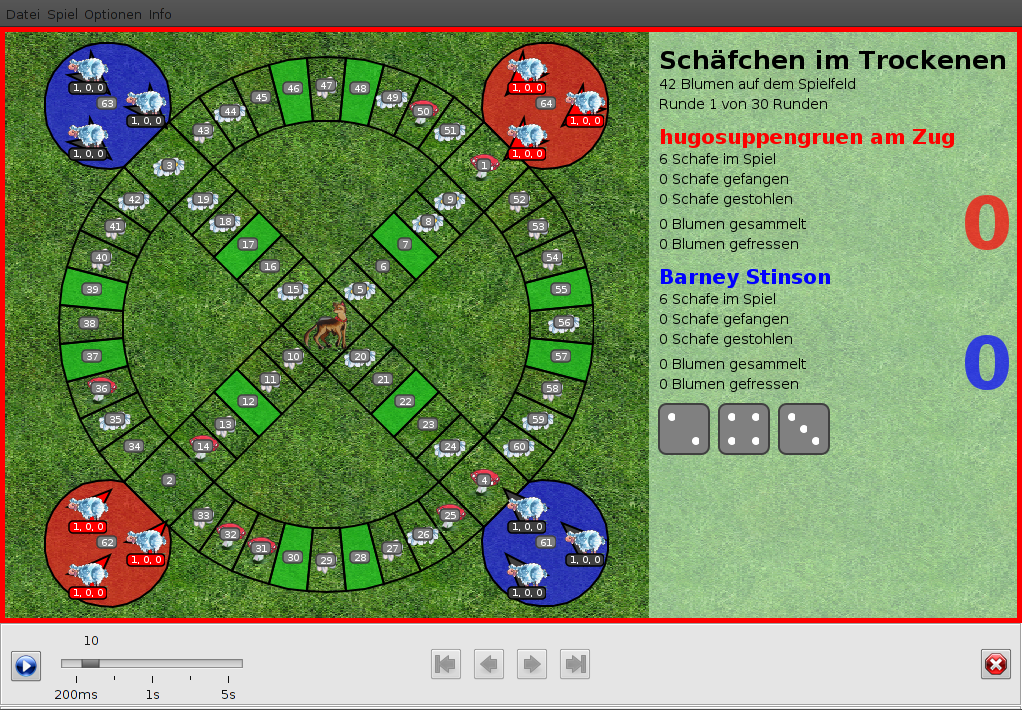
\includegraphics[width=0.75\paperwidth]{ps/server}

\vspace*{-0.2cm}


\vfill{}
 Stand: 31.08.2010 \tableofcontents{}


\chapter*{,,Sch\"{a}fchen im Trockenen{}``}


\section{Einf\"{u}hrung}

Bei ,,Sch\"{a}fchen im Trockenen{}`` spielen zwei Spieler darum,
die gr\"{o}\ss{}te Schafherde zu bilden und damit die meisten Punkte
zu sammeln. Der erste Spieler spielt in \textbf{rot}, der zweite Spieler
in \textbf{blau}.

Um die Zufriedenheit der Herde zu steigern, k\"{o}nnen die Schafe
auf dem Spielplan leckere Blumen \textbf{sammeln}. Vor unbek\"{o}mmlichen
Fliegenpilzen sollten sie sich aber fernhalten. Sie k\"{o}nnen auch
Schafe des Gegenspielers \textbf{fangen} und dessen Blumen und Fliegenpilze
\"{u}bernehmen. Wenn sie den \textbf{Sch\"{a}ferhund} dabei haben,
gelingt ihnen dies noch \"{o}fter.

\textbf{Schafe} bilden durch das Fangen von gegnerischen Schafen \textbf{Schafherden}.
Im Folgenden werden die Begriffe gleichwertig verwendet. Eine Schafherde
wird immer durch das eine Schaf identifiziert, das die restliche Herde
eingefangen hat. Kommt eine Schafherde nach Hause, werden die gesammelten
Blumen \textbf{gefressen} und die gefangenen Schafe \textbf{gestohlen},
das hei\ss{}t endg\"{u}ltig aus dem Spiel entfernt.

Gespielt wird auf einem Spielplan, der immer gleich aufgebaut ist.
Die Positionen der Blumen und Fliegenpilze wechseln jedoch von Spiel
zu Spiel. Die W\"{u}rfel entscheiden, wie weit sich ein Schaf in einem
Spielzug bewegen kann.


\section{Spielmaterial}


\subsection{Spielplan}

%
\begin{figure}[H]
\begin{centering}
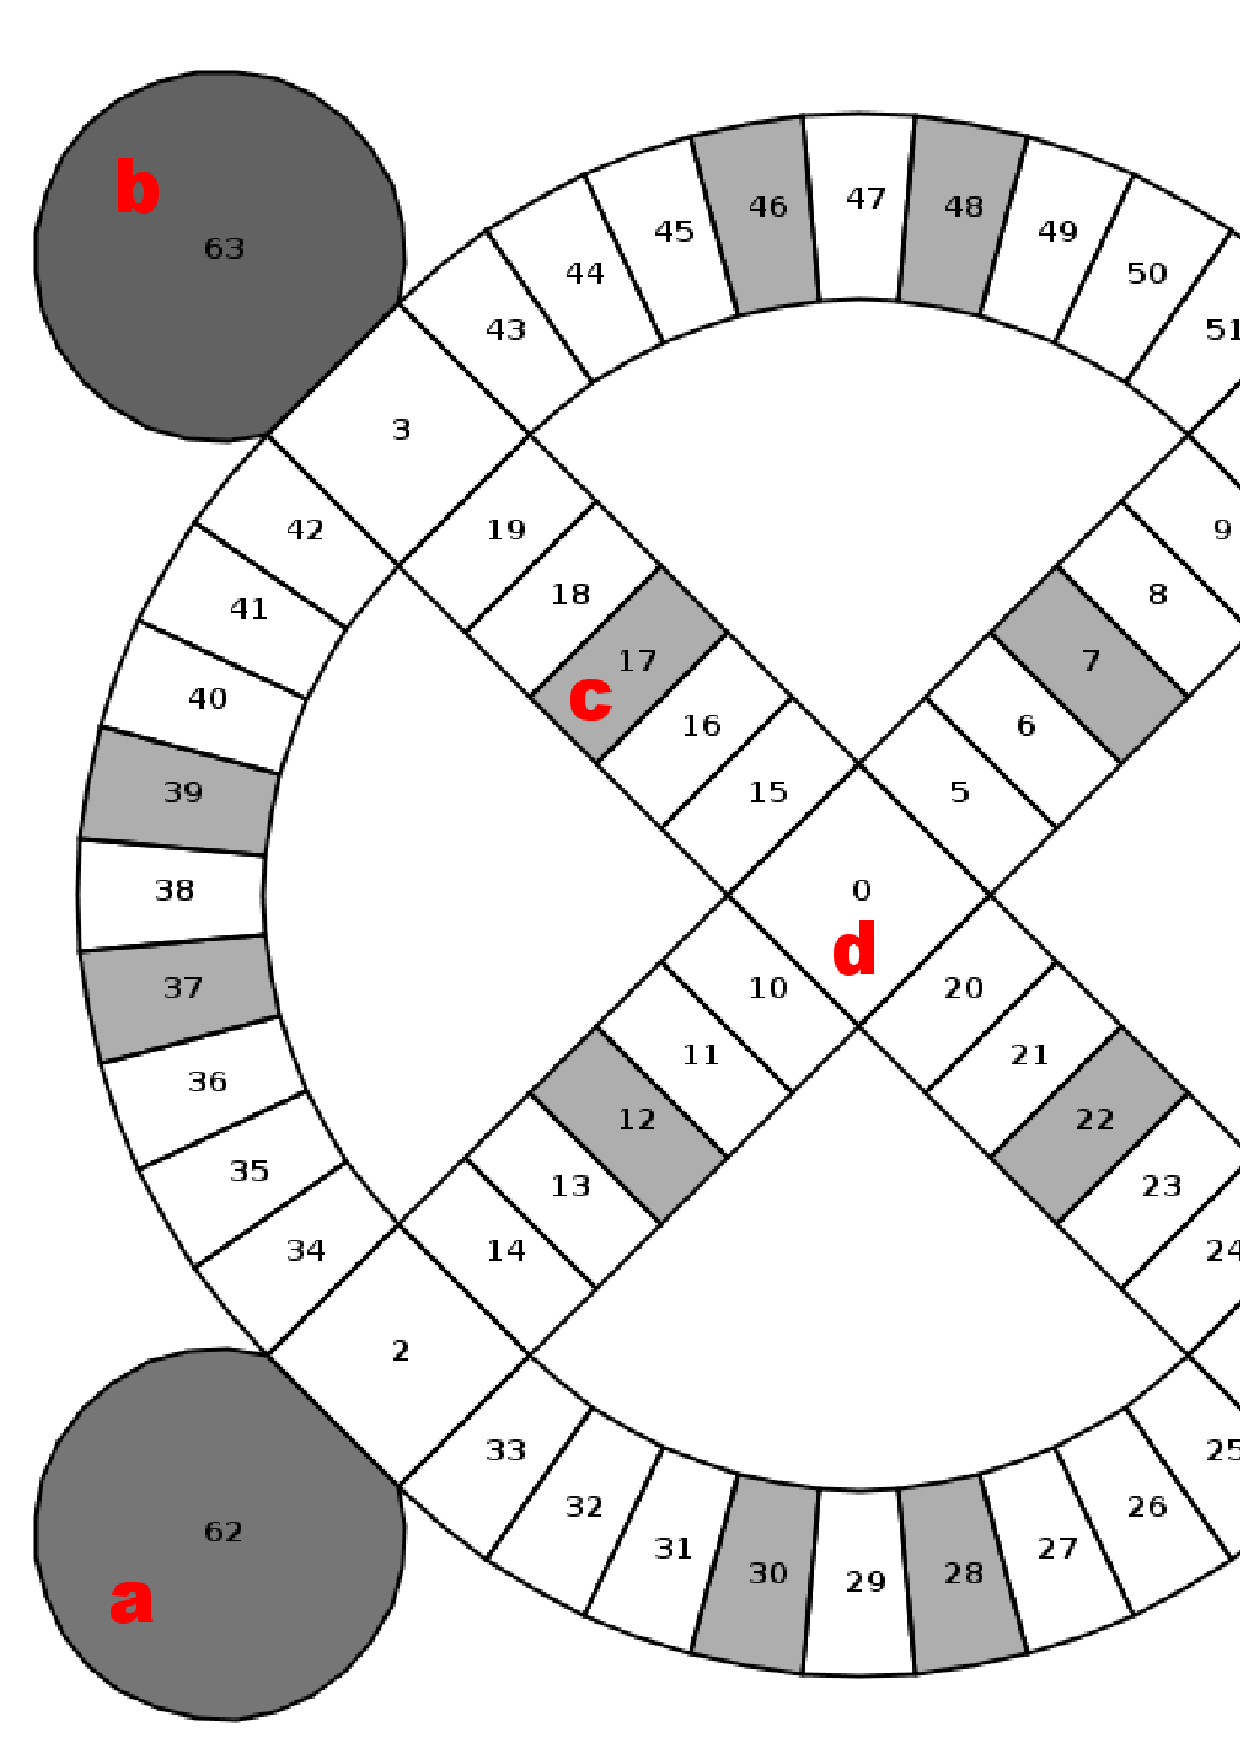
\includegraphics[width=0.5\paperwidth]{ps/spielplan}
\par\end{centering}

\caption{Der Spielplan mit den Indizes der Spielfelder. Markiert sind a) die
Heimatfelder des ersten Spielers, b) die Heimatfelder des zweiten
Spielers, c) ein Sicherheitsfeld und d) ein normales Feld.}


\label{spielplan} 
\end{figure}


Der Spielplan besteht aus 65 Spielfeldern und ist immer gleich aufgebaut,
s. Abbildung \ref{spielplan}. Jedes Schaf befindet sich immer auf
genau einem Spielfeld und im Allgemeinen darf auf jedem Spielfeld
immer nur ein Schaf stehen. Jedes Spielfeld hat einen eindeutigen
Index.

Es gibt drei verschiedene Sorten von Feldern auf dem Spielplan:
\begin{itemize}
\item \textbf{Heimatfelder}: Hier befinden sich die Schafe zu Beginn des
Spiels. Die Schafe betreten ihre Heimatfelder gerne, denn nur hier
k\"{o}nnen sie ungest\"{o}rt fressen und gefangene Schafe stehlen.
Jeder Spieler besitzt zwei gegen\"{u}berliegende Heimatfelder. Dies
sind die einzigen Felder, auf denen mehr als ein Schaf gleichzeitig
stehen kann.
\item \textbf{Sicherheitsfelder}: Auf diesen Feldern ist ein Schaf relativ
sicher. Es kann nur dann vom Gegenspieler gefangen werden, wenn sein
Schaf den aktiven Sch\"{a}ferhund dabei hat.
\item \textbf{Normale Felder}: Auf diesen Feldern k\"{o}nnen sich die Blumen
und Fliegenpilze befinden. Sie werden von dem ersten Schaf, das ein
solches Feld betritt, automatisch eingesammelt und mitgenommen. 
\end{itemize}
Die Schafe finden die \textbf{Blumen} sehr lecker und sollten so viele
Blumen wie m\"{o}glich sammeln und sp\"{a}ter fressen. Dies macht
die Schafe gl\"{u}cklich und bringt dem Spieler Punkte.

Zus\"{a}tzlich zu den Blumen befinden sich auf dem Spielplan auch
\textbf{Fliegenpilze}.

Auch diese werden gesammelt, wenn ein Schaf ein entsprechendes Feld
betritt und sp\"{a}ter gefressen. Allerdings gilt es, die Fliegenpilze
zu vermeiden, denn sie bekommen den Schafen nicht gut und z\"{a}hlen
daher \textbf{negativ}.

%
\begin{figure}[!h]
\begin{centering}

\includegraphics[scale=0.75]{ps/blumen}
\par\end{centering}

\caption{Symbole f\"{u}r a) eine Blume, b) zwei Blumen und c) ein Fliegenpilz.}


\label{blumen} 
\end{figure}



\subsection{Spielfiguren}

Jedes \textbf{Schaf} ist genau einem der beiden Spieler zugeordnet
und hat einen eindeutigen Index. Im Spiel wird jedes Schaf durch eine
Spielfigur in der Farbe seines Spielers dargestellt. Die Spielfiguren
des Spielers, der nicht am Zug ist, werden grau dargestellt.

Ein Schaf kann im Laufe des Spiels gegnerische Schafe fangen bzw.
in seine Herde aufnehmen. Hatte ein gegnerisches Schaf schon Schafe
gefangen, k\"{o}nnen so auch eigene Schafe in die Herde gelangen,
sie werden also \textbf{zur\"{u}ckgefangen}. Wie bereits erw\"{a}hnt,
kann jedes Schaf Blumen oder Fliegenpilze sammeln.

%
\begin{figure}[H]
\begin{centering}
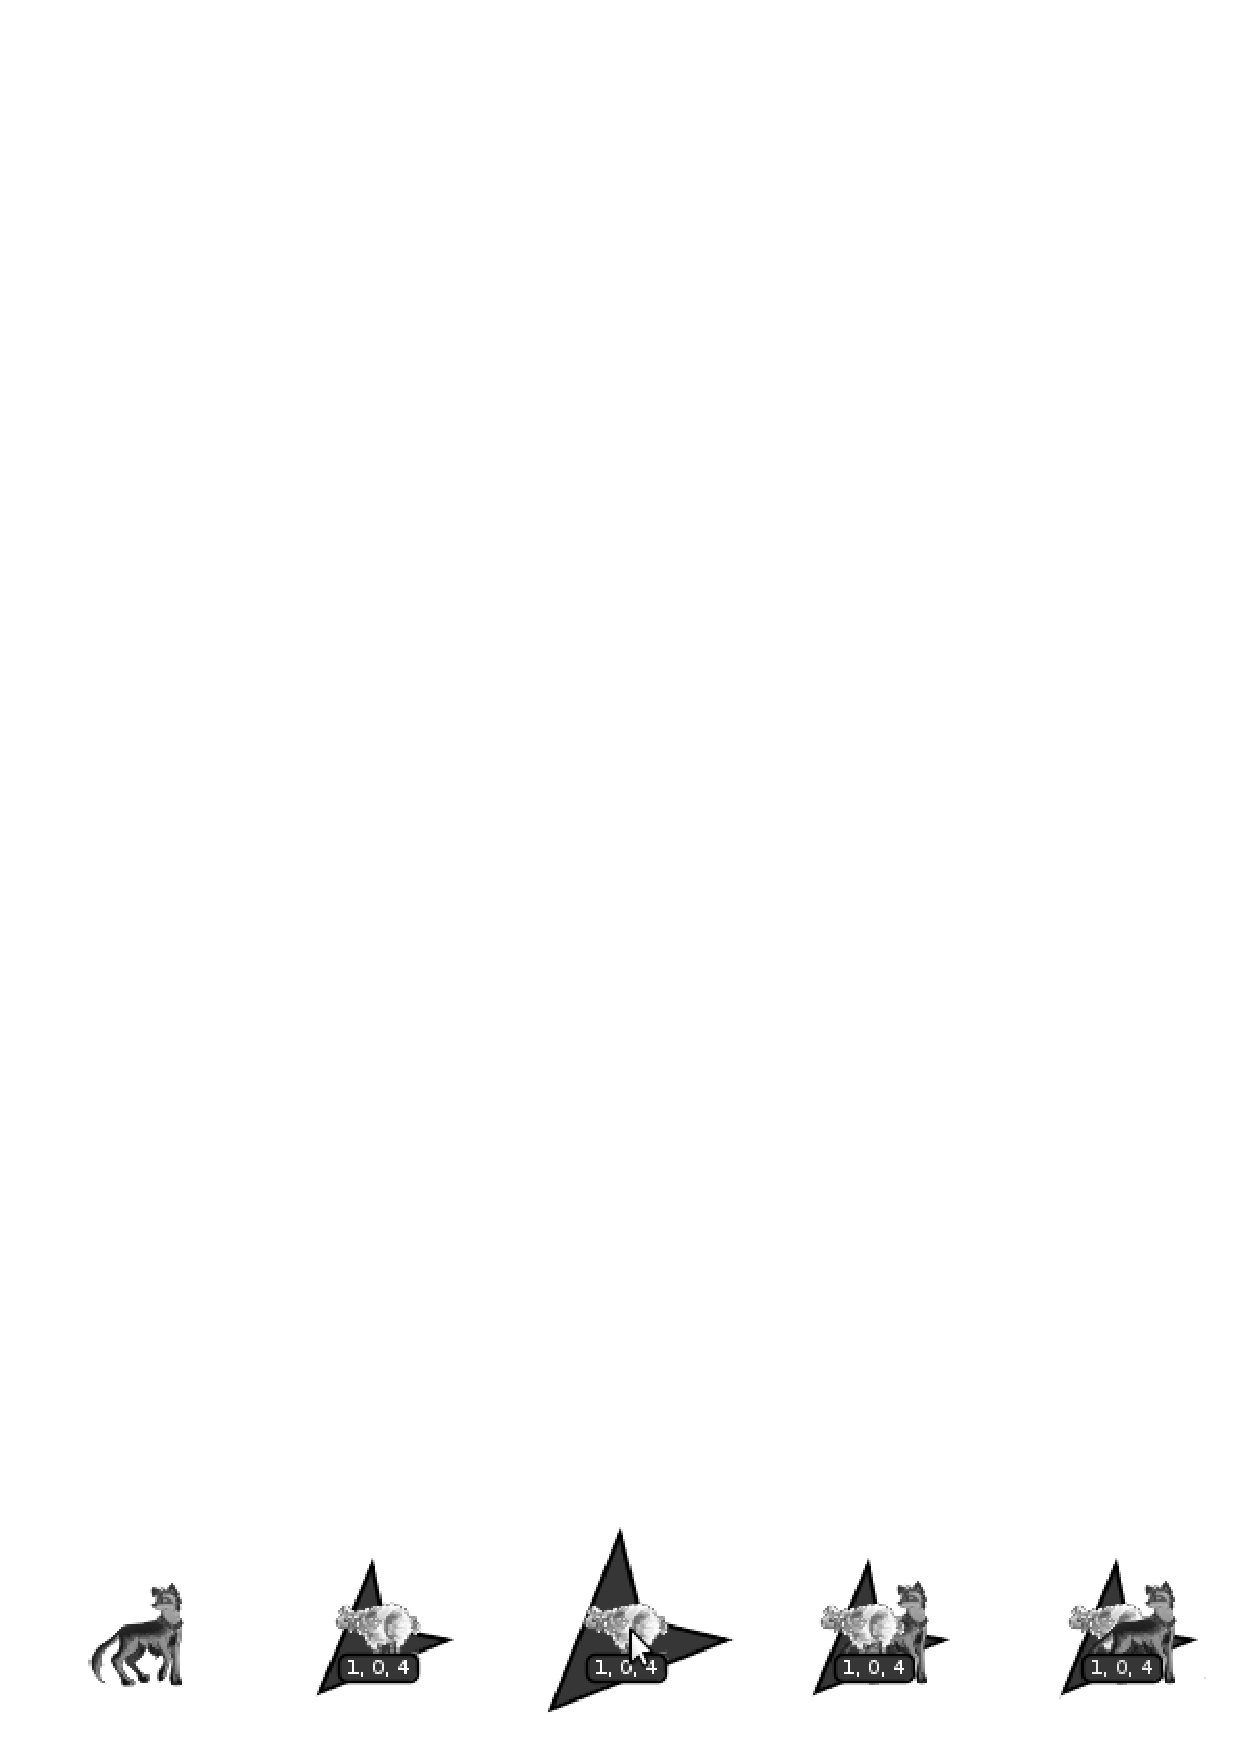
\includegraphics[scale=0.4]{ps/schafe}
\par\end{centering}

\caption{Die Spielfiguren f\"{u}r a) den Sch\"{a}ferhund zu Beginn, b) ein
Schaf c), ein mit der Maus bewegtes Schaf, d) ein Schaf mit passivem
Sch\"{a}ferhund und e) ein Schaf mit aktivem Sch\"{a}ferhund.}


\label{schafe} 
\end{figure}


Die drei Zahlen nunter den Spielfiguren haben der Reihe nach folgende
Bedeutung: 
\begin{itemize}
\item Die Anzahl der \textbf{eigenen Schafe} inklusive des Schafes, das
durch diese Spilfigur symbolisiert wird. Diese Zahl kann daher nie
kleiner als 1 sein. 
\item Die Anzahl der gefangenen, \textbf{gegnerischen Schafe}. Diese Zahl
kann nie kleiner als 0 sein. 
\item Die Anzahl der gesammelten Blumen abz\"{u}glich der Anzahl der gesammelten
Fliegenpilze. Diese Zahl kann also auch negativ sein. 
\end{itemize}
Ein Schaf darf nach dem Verlassen eines Heimatfeldes nur das Heimatfeld
betreten, das dem \textbf{von ihm zuletzt verlassenen} Heimatfeld
\textbf{gegen\"{u}berliegt}. Unter der Spielfigur befindet sich ein
Pfeil, der immer auf dieses Heimatfeld zeigt. Wird eine Spielfigur
mit der Maus bewegt, wird der Pfeil etwas gr\"{o}\ss{}er.

Zus\"{a}tzlich zu den Schafen gibt es genau einen \textbf{Sch\"{a}ferhund}.
Ein Schaf, das auf das Feld mit dem Sch\"{a}ferhund zieht, wird fortan
von diesem \textbf{begleitet}. Wird ein von dem Sch\"{a}ferhund begleitetes
Schaf von einem anderen Schaf gefangen, so begleitet der Sch\"{a}ferhund
ab sofort das neue Schaf. Ist der Sch\"{a}ferhund also einmal mitgenommen
worden, begleitet er von da an immer ein Schaf.

Zu Beginn des Spiels ist der Sch\"{a}ferhund \textbf{passiv}. Er wird
\textbf{aktiv}, wenn er das erste Mal von einem Schaf mit \textbf{in
ein Heimatfeld genommen} wird. Erst jetzt hat er einen Nutzen, denn
er erlaubt es von da an dem von ihm begleiteten Schaf, auch gegnerische
Schafe auf \textbf{Sicherheitsfeldern} zu fangen. Er besch\"{u}tzt
ein Schaf aber \textbf{nicht} davor, selbst gefangen zu werden. Ist
der Sch\"{a}ferhund einmal aktiv geworden, wird er nie wieder passiv.


\subsection{W\"{u}rfel}

Im Spiel gibt es drei W\"{u}rfel mit Augenzahlen zwischen 1 und 6.
Eine Augenzahl gibt an, um wieviele Felder sich ein Schaf in einem
Zug bewegen kann. Der W\"{u}rfelvorrat wird von beiden Spielern gemeinsam
benutzt und jedem Schaf steht jeder W\"{u}rfel zur Verf\"{u}gung.
Der Spieler muss sich aber f\"{u}r ein Schaf und eine der vorhandenen
Augenzahlen entscheiden.

Sobald ein Spieler eine Augenzahl genutzt hat, wird ein W\"{u}rfel
mit dieser Augenzahl neu gew\"{u}rfelt. Der Wurf wird solange wiederholt,
bis die folgenden beiden Bedingungen erf\"{u}llt sind:
\begin{itemize}
\item Dem Spieler m\"{u}ssen zu jedem Zeitpunkt mindestens zwei verschiedene
Augenzahlen zur Verf\"{u}gung stehen. 
\item Der Spieler, der als n\"{a}chstes am Zug ist, muss mindestens einen
g\"{u}ltigen Zug machen k\"{o}nnen. 
\end{itemize}

\section{Spielbeginn}

Jeder Spieler beginnt mit \textbf{sechs} einzelnen Schafen, je drei
in den beiden gegen\"{u}berliegenden Heimatfeldern. Der Sch\"{a}ferhund
befindet sich zun\"{a}chst in der Mitte des Spielplans auf dem Feld
mit dem Index 0.

Zu Spielbeginn befinden sich je ein Fliegenpilz auf \textbf{acht}
zuf\"{a}llig gew\"{a}hlten, normalen Feldern und \textbf{f\"{u}nfzig}
Blumen auf den \"{u}brigen normalen Feldern. Dabei sind jedoch nie
mehr als zwei Blumen auf einem Feld. Es kann normale Felder geben,
auf denen sich weder Blumen noch Fliegenpilze befinden.

Alle drei W\"{u}rfel wurden unter Einhaltung der beiden zuvor genannten
Bedingungen gew\"{u}rfelt.


\section{Spielablauf}

Das Spiel ist rundenbasiert. In jeder Runde bewegt zun\"{a}chst der
erste Spieler eines seiner Schafe auf ein Feld, auf das dieses Schaf
ziehen darf. Wie wit ein Schaf ziehen kann, richtet sich generell
nach den Augenzahlen der W\"{u}rfel (stehen z.B. die Augenzahlen 2,
2, 5 zur Verf\"{u}gung, darf ein Schaf 2 oder 5 Felder weit ziehen).

Dabei ist zu beachten, dass in den folgenden F\"{a}llen ein Schaf
ein Spielfeld nicht betreten darf:
\begin{itemize}
\item Wenn es sich um ein gegnerisches Heimatfeld handelt. 
\item Wenn es sich um das eigene Heimatfeld handelt, das von dem Schaf zuletzt
verlassen wurde.
\item Wenn es sich um ein Sicherheitsfeld handelt, auf dem ein eigenes Schaf
steht. 
\item Wenn es sich um ein Sicherheitsfeld handelt, auf dem ein gegnerisches
Schaf steht und das sich bewegende Schaf nicht in Begleitung des aktiven
Sch\"{a}fer\-hundes ist.
\item Wenn es sich um ein normales Feld handelt, auf dem bereits ein eigenes
Schaf steht. 
\end{itemize}
Nachdem der erste Spieler seinen Zug beendet hat, wird ein W\"{u}rfel
mit der verwendeten Augenzahl den Regeln entsprechend neu gew\"{u}rfelt.
Anschlie\ss{}end macht auch der zweite Spieler einen solchen Zug und
es wird erneut gew\"{u}rfelt. Damit ist eine Runde beendet.


\subsection{Schafe bewegen}

Wird im Spiel eine Spielfigur mit der Maus bewegt, werden alle Felder,
auf die das zugeh\"{o}rige Schaf ziehen darf, mit einem Rahmen \textbf{hervorgehoben}.
Die Farbe des Rahmens entspricht der Farbe der Spielfigur. Auch eine
Spielfigur des Spielers, der momentan nicht am Zug ist, kann mit der
Maus bewegt werden. So kann man sich angucken, welche Felder ein Schaf
theoretisch betreten k\"{o}nnte, wenn sein Spieler bereits am Zug
w\"{a}re.

Zieht man eine Spielfigur des aktuellen Spielers \"{u}ber ein hervorgehobenes
Spielfeld, so wird dieses Feld zus\"{a}tzlich mit der Farbe der Spielfigur
\textbf{hinterlegt}. L\"{a}sst man die Spielfigur \"{u}ber einem so
hinterlegten Feld los, bewegt sich das Schaf auf dieses Feld.

Abbildung \ref{spielzug} zeigt, wie ein kompletter Spielzug im Spiel
aussieht.

%
\begin{figure}[!h]
\begin{centering}
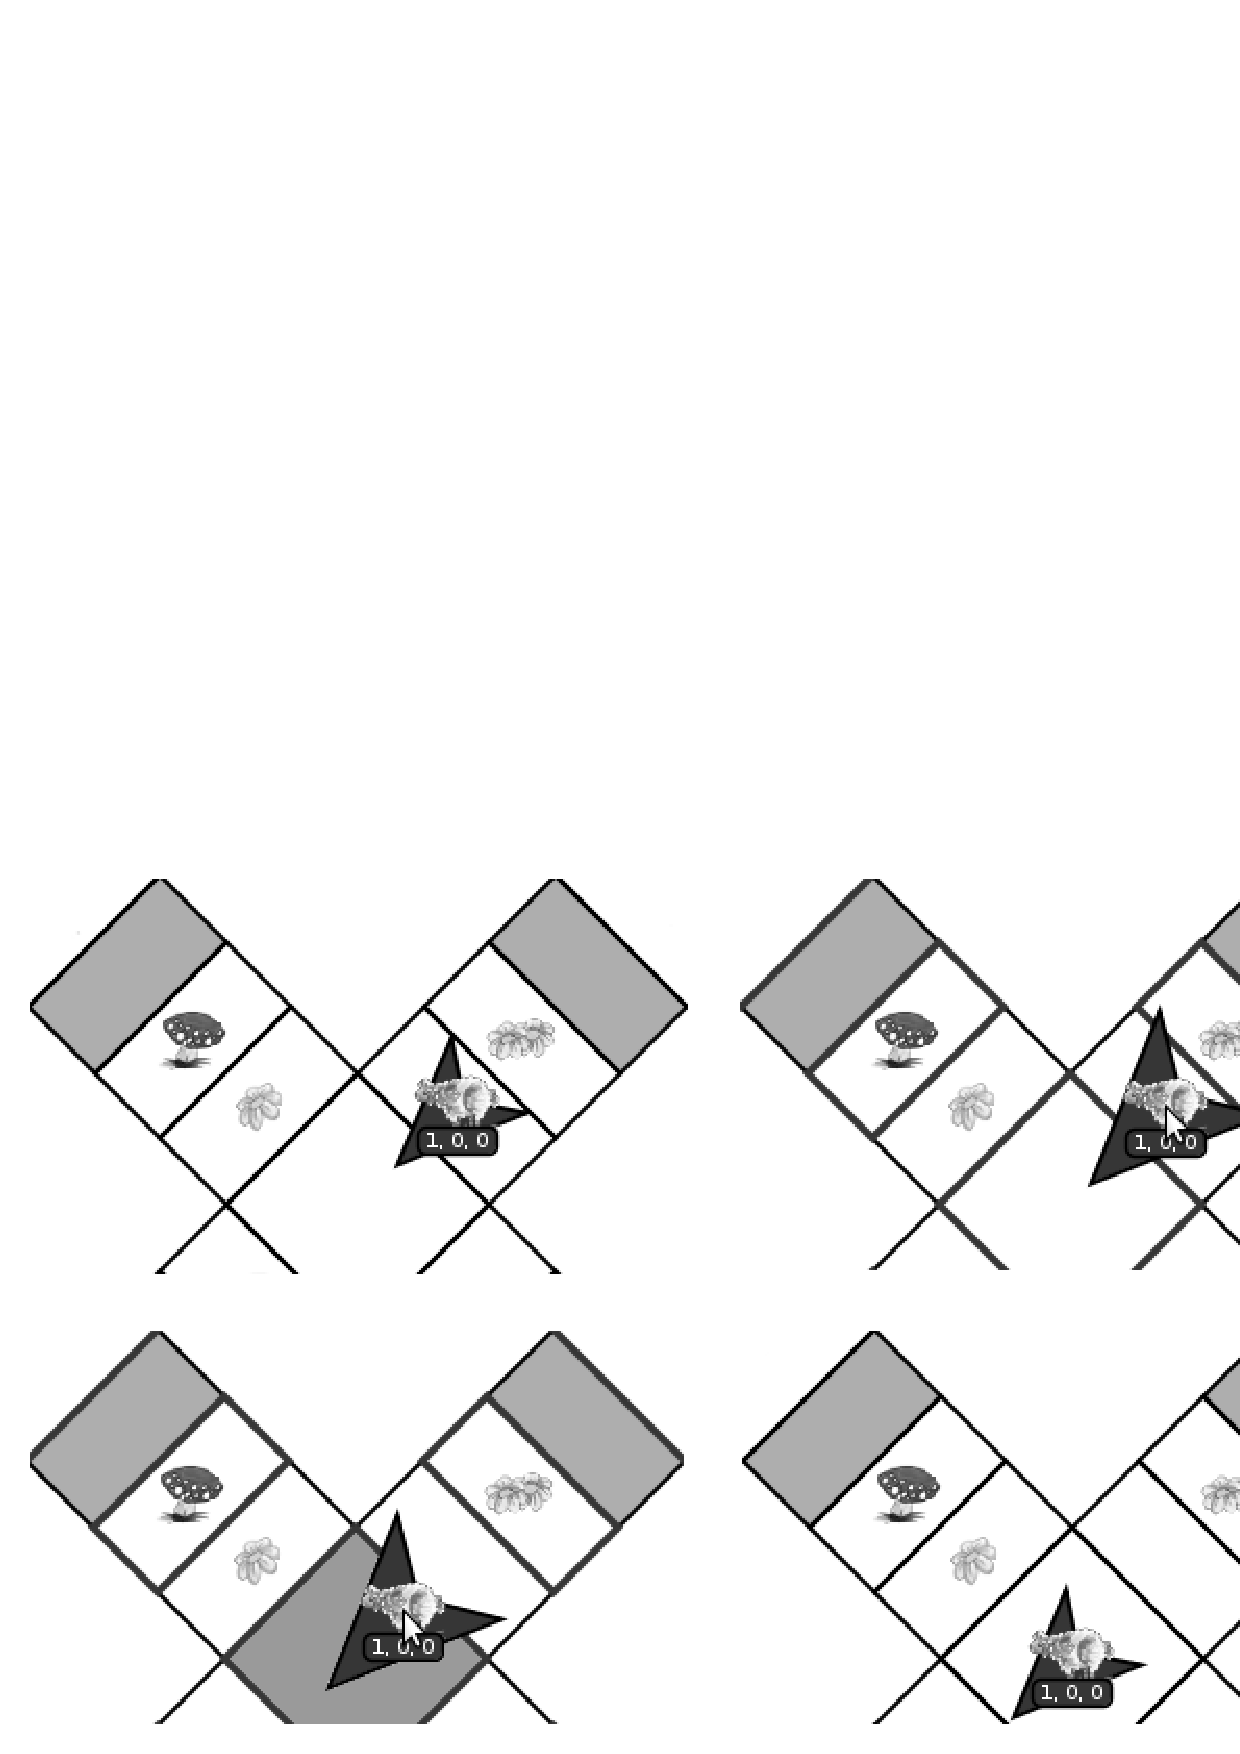
\includegraphics[scale=0.4]{ps/spielzug}
\par\end{centering}

\caption{Eine Spielfigur auf dem Spielplan a) vor dem Spielzug, b) mit hervorgehobenen
Spielfeldern, c) mit hinterlegtem Spielfeld und d) nach dem Spielzug.}


\label{spielzug} 
\end{figure}



\subsection{Nach der Bewegung}

Bewegt sich ein Schaf auf ein Feld, werden alle dort vorhandenen Blumen
und Fliegenpilze eingesammelt.

Befindet sich ein gegnerisches Schaf auf dem Spielfeld, wird dieses
Schaf gefangen. Alle von diesem nun gefangenen Schaf bereits gefangenen
Schafe und eingesammelten Blumen und Fliegenpilze werden \"{u}bernommen.

Wird ein Heimatfeld betreten, frisst das heimgekehrte Schaf alle von
ihm gesammelten Blumen und Fliegenpilze. Der Spieler erh\"{a}lt f\"{u}r
gegnerische Schafe sowie gefressene Blumen und Fliegenpilze Punkte
(s. Kapitel 5). Alle nach Hause gebrachten Blumen und Fliegenpilze
sowie Schafe werden aus dem Spiel entfernt%
\footnote{Die mitgebrachten, eigenen Schafe werden aus Implementierungsgr\"{u}nden
nicht befreit. Er werden tats\"{a}chlich neue Schafe erstellt. Diese
haben auch einen neuen, vorher nicht vergebenen Index.%
}. Dabei ist folgendes zu beachten:
\begin{itemize}
\item Handelte es sich um ein gegnerisches, also ein \textbf{gefangenes}
Schaf, ist es endg\"{u}ltig aus dem Spiel raus. Es ist nun \textbf{gestohlen}. 
\item Handelte es sich um ein eigenes, also ein \textbf{zur\"{u}ckgefangenes}
Schaf, wird in dieses Heimatfeld ein neues, eigenes Schaf gestellt. 
\end{itemize}
Nach einer Bewegung kann in einem Heimatfeld also niemals ein Schaf
stehen, das von weiteren Schafen begleitet wird.


\section{Punkte}

Spielbegleitend werden Punkte nach den folgenden Regeln verteilt:
\begin{itemize}
\item F\"{u}r jede gesammelte Blume gibt es zwei Punkte. 
\item F\"{u}r jeden gesammelten Fliegenpilz gibt es zwei Minuspunkte. 
\item F\"{u}r jede gefressene Blume gibt es zwei zus\"{a}tzliche Punkte. 
\item F\"{u}r jeden gefressenen Fliegenpilz gibt es zwei zus\"{a}tzliche
Minuspunkte. 
\item F\"{u}r jedes gefangene, gegnerische Schaf gibt es acht Punkte. 
\item F\"{u}r jedes gestohlene, gegnerische Schaf gibt es acht zus\"{a}tzliche
Punkte. 
\end{itemize}

\section{Spielende}

Das Spiel endet, sobald ein Spieler keine Schafe mehr hat; sp\"{a}testens
aber nach 30 Runden.

Ist das Spiel vorzeitig zu Ende, gewinnt der Spieler, der als einziger
noch ein Schaf hat. Werden alle 30 Runden gespielt, gewinnt der Spieler
mit mehr Punkten. Bei gleichem Punktestand ist das Spiel unentscheiden.


\section{Weitere Elemente}

Um das Spielfeld herum ist immer ein Rahmen in der Farbe des aktuellen
Spielers gezeichnet.

An der rechten Seite befindet sich die in Abbildung \ref{seitenleiste}
gezeigte Seitenleiste mit einigen Spielinformationen. Sie zeigt, wie
viele Blumen noch auf dem Spielfeld vorhanden sind. Von diesem Wert
ist die Anzahl der noch vorhandenen Fliegenpilze bereits abgezogen,
so dass zu Beginn des Spiels hier 42 steht. Darunter wird angezeigt,
in der wievielten Runde sich das Spiel befindet.

In der normalen Ansicht werden darunter f\"{u}r beide Spieler einige
Statusinformationen gezeigt. In der Debugansicht sind dieselben Informationen
in einer kompakten Darstellung zu finden.

%
\begin{figure}[!t]
\begin{centering}
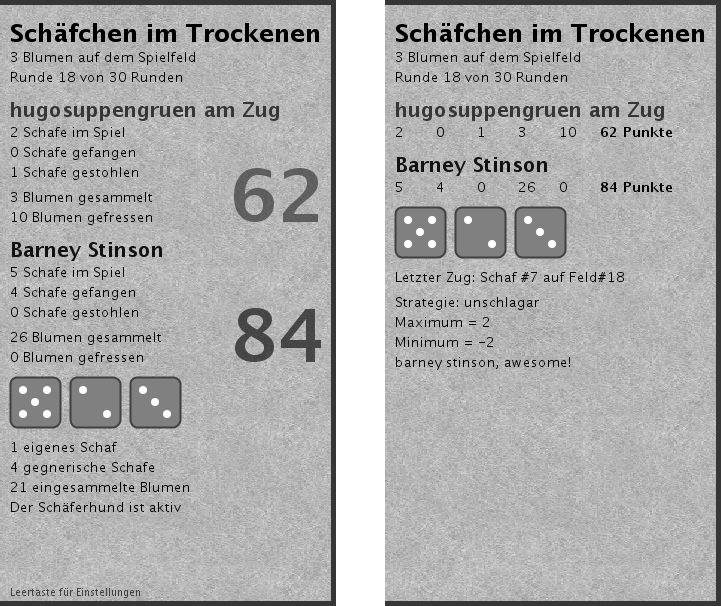
\includegraphics[scale=0.5]{ps/seitenleiste}
\par\end{centering}

\caption{Die Seitenleiste in \protect \\
a) normaler Ansicht oder \protect \\
b) Debugansicht zeigt \protect \\
c) den aktuellen Spielstand, \protect \\
d) ausf\"{u}hrliche Spielerinformation bzw. \protect \\
e) kompakte Spielerinformation, \protect \\
f) die vorhandenen Augenzahlen, \protect \\
g) Informationen \"{u}ber eine markierte Spielfigur, \protect \\
h) der letzte Spielzug, \protect \\
i) Debuginformationen und \protect \\
j) Hinweis auf das Einstellungsmen\"{u}.}


\label{seitenleiste} 
\end{figure}


Zudem werden die momentan verf\"{u}gbaren Augenzahlen der drei W\"{u}rfel
angezeigt.

Wird eine Spielfigur mit der Maus bewegt, werden in der normalen Ansicht
nochmals die wichtigsten Informationen \"{u}ber diese Spielfigur angezeigt.
In der Debugansicht werden die Kenndaten des letzten Zuges eingeblendet.
Darunter befinden sich gegebenenfalls von einem Client gesendete Debuginformationen.

Hat das Spielfeld den Tastaturfokus, erscheint unten ein Hinweis auf
das Einstellungsmen\"{u}. Um dem Spielfeld den Fokus zu geben, muss
man ggf. einmal in das Spielfeld klicken. Hat das Spielfeld den Fokus,
kann mit der \textbf{Leertaste} das in Abbildung \ref{einstellungen}
gezeigte Men\"{u} ge\"{o}ffnet und wieder geschlossen werden.

%
\begin{figure}[!t]
\begin{centering}
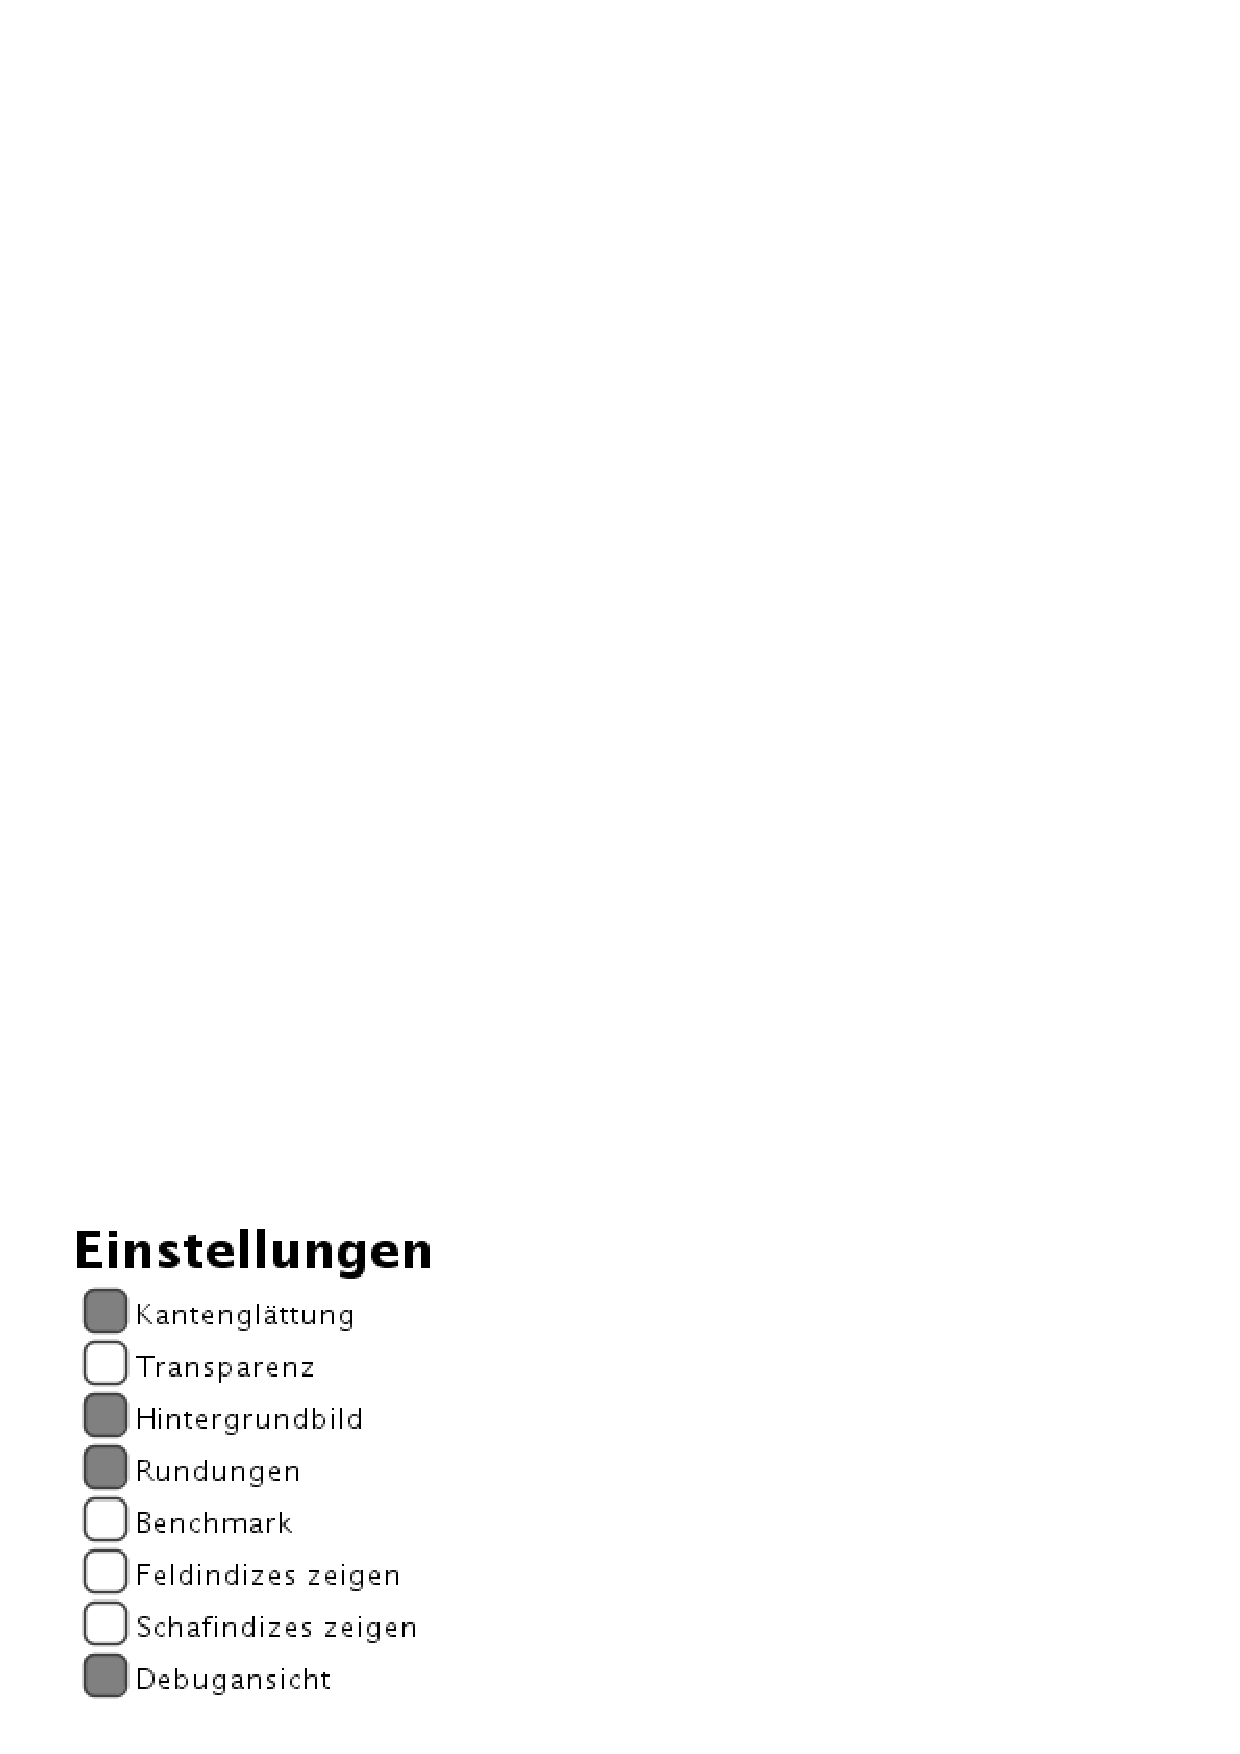
\includegraphics[scale=0.75]{ps/einstellungen}
\par\end{centering}

\caption{Das Einstellungsmen\"{u}.}


\label{einstellungen} 
\end{figure}


Die Optionen \textbf{Kantengl\"{a}ttung}, \textbf{Transparenz}, \textbf{Hintergrundbild}
und \textbf{Rundungen} beeinflussen die grafische Darstellung des
Spiels. Insbesondere die ersten beiden Optionen sind sehr rechenintensiv
und sollten auf schw\"{a}cheren Rechnern ausgeschaltet werden. Mit
der Option \textbf{Benchmark} kann \"{u}berpr\"{u}ft werden, ob die
momentanen Einstellungen f\"{u}r den Rechner geeignet sind.

\"{U}ber die Optionen \textquotedbl{}\textbf{Feld--} und \textbf{Schafindizes
zeigen}\textquotedbl{} kann \"{u}ber jedem Feld bzw. Schaf der zugeh\"{o}rige,
eindeutige Index eingeblendet werden.

Die Option \textbf{Debugansicht} legt fest, welche Seitenleiste angezeigt
werden soll.
\end{document}
